The yield model results with optimal threshold levels, as well as the estimated values of the threshold parameters, will be presented. The relationship between precipitation and yield during the approximate time where silking and pollination occurs was modelled  as a piecewise linear function. This relationship was modelled with two separate threshold points. The constrained case where the second threshold coefficient is set equal to the first, thereby collapsing the model to a single threshold model was also considered. Spatial autocorrelation was dealt with using a spatial weighting matrix which indicates neighbouring counties' observations within the same time period. The spatial correlation parameter $\rho$ was estimated by maximizing a likelihood function with respect to this parameter. As the maximizing value can not be exactly solved algebraically, this maximization was accomplished using the optim function in R, but could also be done through a direct manual search on potential values of $\rho$. The maximization of the likelihood function needed to determine the optimal spatial correlation parameter $\rho$ for a particular model is very time consuming. Two method variations were considered for the estimation of the yield models. The first method assumes that the optimal value for the spatial correlation parameter would depend on the threshold levels. In this method the optimal spatial correlation parameter was recalculated for every combination of threshold parameters considered. This method is very computationally expensive, as the likelihood function must be optimized for $\rho$ given each potential set of threshold parameters, and limits the number of different parameter combinations that can be tested. The second method assumed that the threshold levels would not have a significant effect on the optimal spatial correlation parameter. The optimal spatial correlation parameter was estimated with the threshold variables omitted; this value was then used for the model estimation given each combination of threshold parameters considered. This was done to consider how robust the results would be to a simplification of the model which significantly decreased computing time. Each method was used to estimate the optimal threshold parameters for both the one and two threshold models. This led to four different results for the optimal threshold estimates in each location. The first result was from the method 1 estimation of the two threshold model, the second was from the method 2 estimation of the two threshold model, the third is from the method 1 estimation of the one threshold model, and the fourth is from the method 2 estimation of the one threshold model. Therefore, four results are reported for each location subset with heteroskedastic consistent errors generated using the HC3 option of the hccm function in R. 


\section{Ontario Sub Sections}


Ontario has a varied history of corn production throughout the province and significant climatic differences between the counties included in the study\citep{tolhurst2015cold}. Due to the presence of between county heterogeneity in Ontario, a single model may not be sufficient to accurately describe corn production for all counties included in this study. In general, the following counties: Brant, Chatham-Kent, Elgin, Essex, Haldimand-Norfolk, Lambton, Middlesex and Oxford, in Southern Ontario, have historically had higher average yields in comparison to other counties in the province. These counties are also in close physical proximity to one another. This physical proximity is likely linked to similarities in  farm management practices as well as environmental conditions (for example soil moisture) which are not reflected in the available weather data. These omitted variables are likely to affect yield. On the other hand, certain counties spread throughout the province which were included in our data set have have had relatively low average yields throughout the study period. These counties are Dufferin, Grey, Halton, Hamilton, Hastings, Kawartha Lakes, Lanark, Leeds-Grenville, Lennox-Addington, Niagara, Northumberland, Prince Edward and Renfrew. A ``Corn Producer" subset of Ontario counties was therefore considered in which the counties in this list were excluded. Figure 4.1 shows the average yield over time of all counties in our data set (``All Counties"), the 8 counties included in the Southern Ontario group (``Southern Ontario"), the group of counties with the lowest producers excluded (``Corn Producers"), and the 13 other counties with lower average yield (``Low Producers"). 


\begin{figure}[H]
\centering
 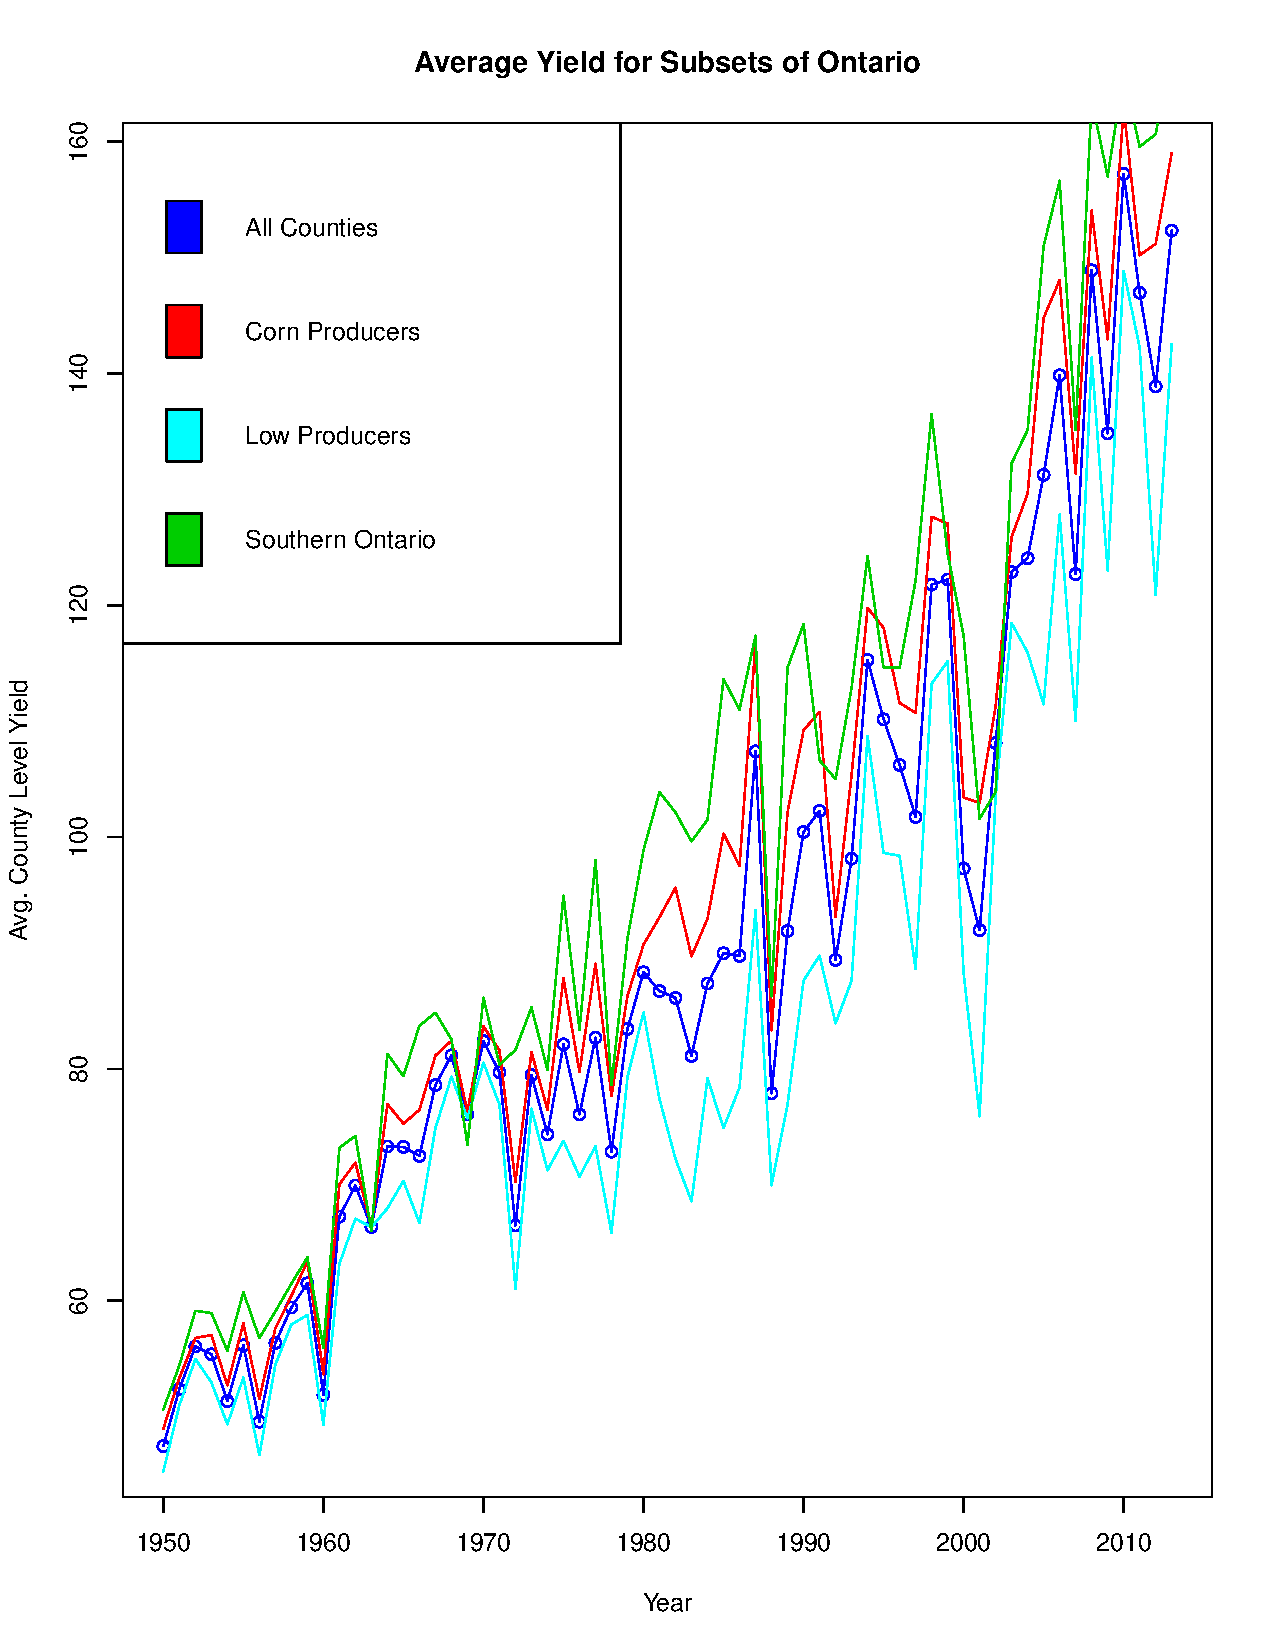
\includegraphics[width=.95\textwidth]{YieldsON.pdf}
    \caption{Plot of Average County level Yield for Subsets of Ontario}
    \end{figure}


Due to the differences in the average county level yields between groups, the yield models were estimated on the ``Southern Ontario" and ``Corn Producers" subsets, in addition to the group including all counties. Another concern results from the climate data used in Ontario. This data comes from environment Canada and was spatially interpolated to county center points. Environment Canada has radar stations spread throughout the province with only 8 radar stations covering the province \citep{EnvirCan}. The counties nearest to these radar stations could have more accurate weather data than the other counties due to this proximity, and could therefore demonstrate the yield climate relationship with higher accuracy. The modelling and determination of threshold levels using only counties nearest to these radar stations was also considered. The counties in question were the following: Huron, Middlesex, Ottawa, Peel, Perth, Prescott-Russel, Stormont-Dundas-Glengarry and York. Results will be presented for the four methods of determining threshold levels for each of these four groups: the entire set of counties, the counties in Southern Ontario, the counties closest to radar stations (``Weather Station Counties"), and the group of counties excluding the 13 less substantial producers. A table will present the relevant regression results for each group.

Iowa is relatively homogeneous in comparison to Ontario. Although there are some climate differences in different regions in the state, most of the counties have been significant producers of corn historically, and Iowa is therefore not subject to the same degree of heterogeneity that Ontario is. All of the counties in Iowa are included in the same model.

\section{Model Results}

The tables below present the model estimates for each location. The model results are from the OLS estimation performed on the transformed data, $Y_{new}$ and $X_{new}$ described in chapter 3, and are presented with robust standard errors (generated using method HC3 in the hccm package in R). In the Ontario model, county specific dummy variables were included, while in Iowa, region specific dummy variables were included. The parameter estimates for these variables are excluded from the tables below for the sake of space.


\begin{table}[H]
    \centering
    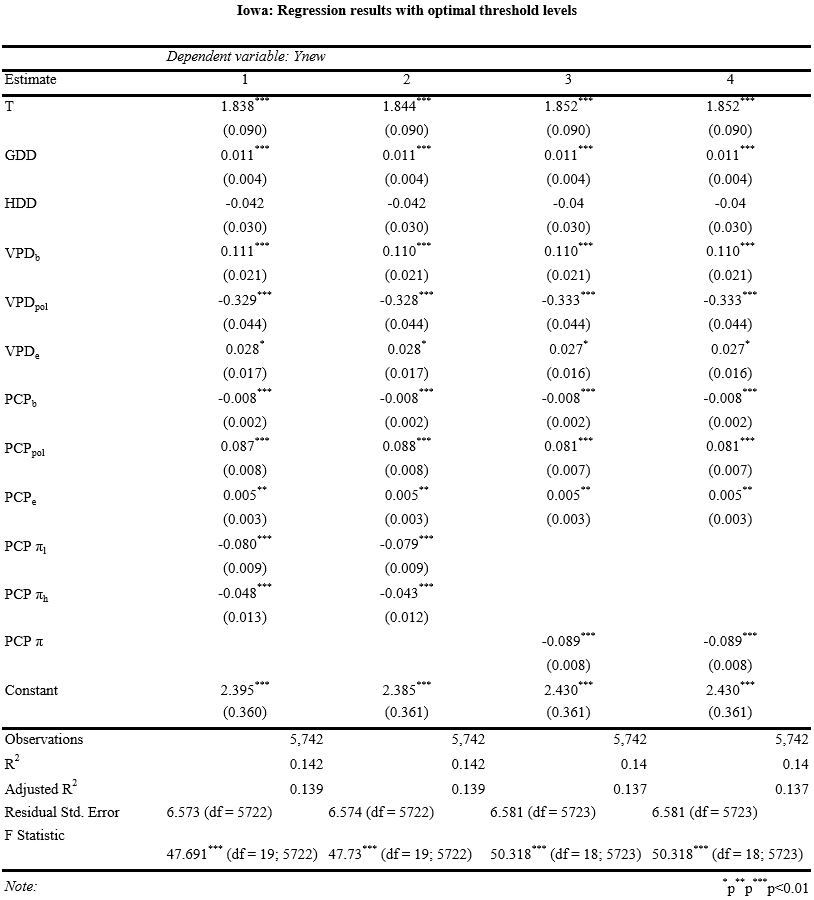
\includegraphics[width=1.0\textwidth]{Iowa_regression_results.png}
    \caption{Iowa: Regression results with optimal threshold levels}
    \label{fig:my_label}
\end{table}

\begin{table}[H]
    \centering
    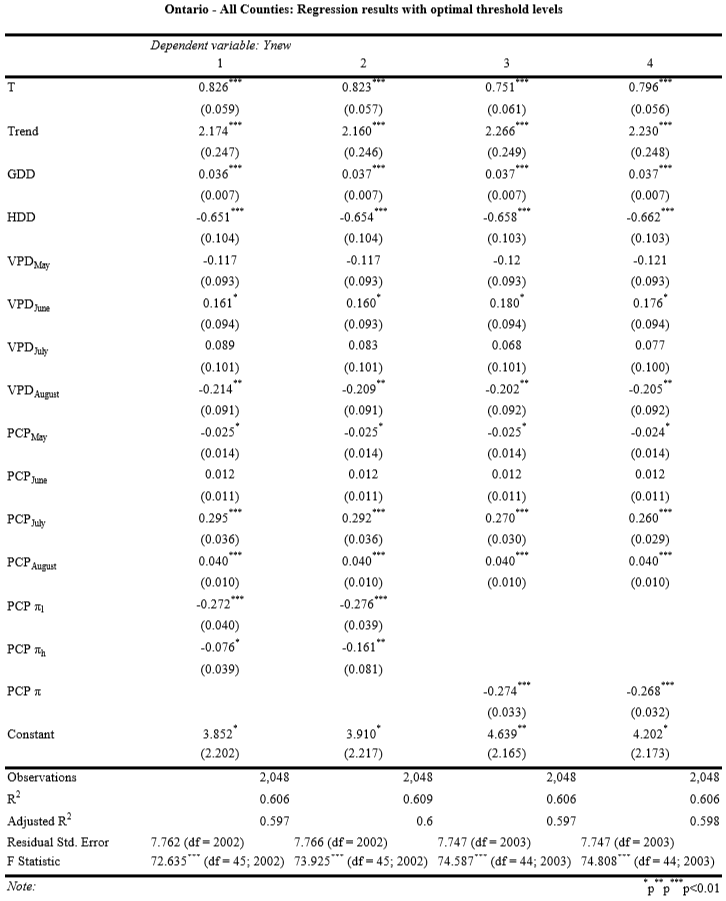
\includegraphics[width=1.0\textwidth]{Ontario_regression_results.png}
    \caption{Ontario - All Counties: Regression results with optimal threshold levels}
    \label{fig:my_label}
\end{table}

\begin{table}[H]
    \centering
    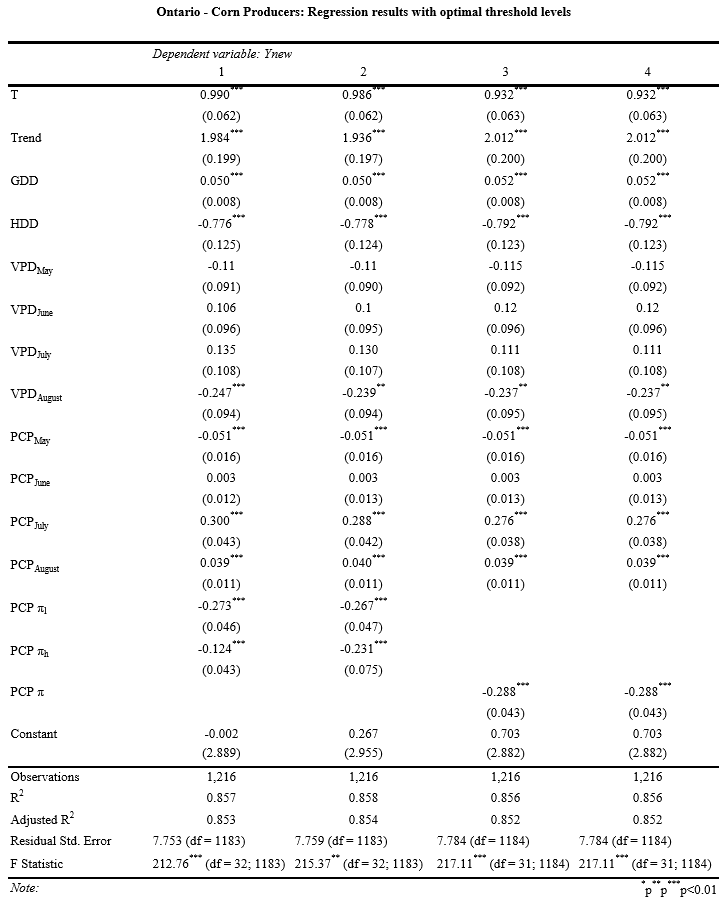
\includegraphics[width=1.0\textwidth]{Ontario_trim_regression_results.png}
    \caption{Ontario - Corn Producers: Regression results with optimal threshold levels}
    \label{fig:my_label}
\end{table}


\begin{table}[H]
    \centering
    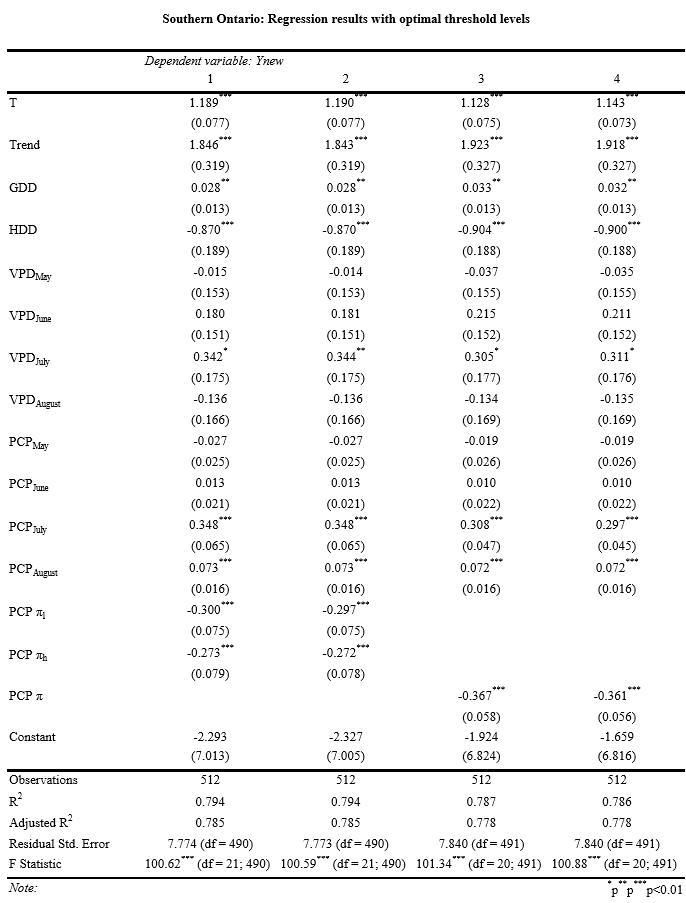
\includegraphics[width=1.0\textwidth]{Ontario_SO_regression_results.png}
    \caption{Southern Ontario: Regression results with optimal threshold levels}
    \label{fig:my_label}
\end{table}


\begin{table}[H]
    \centering
    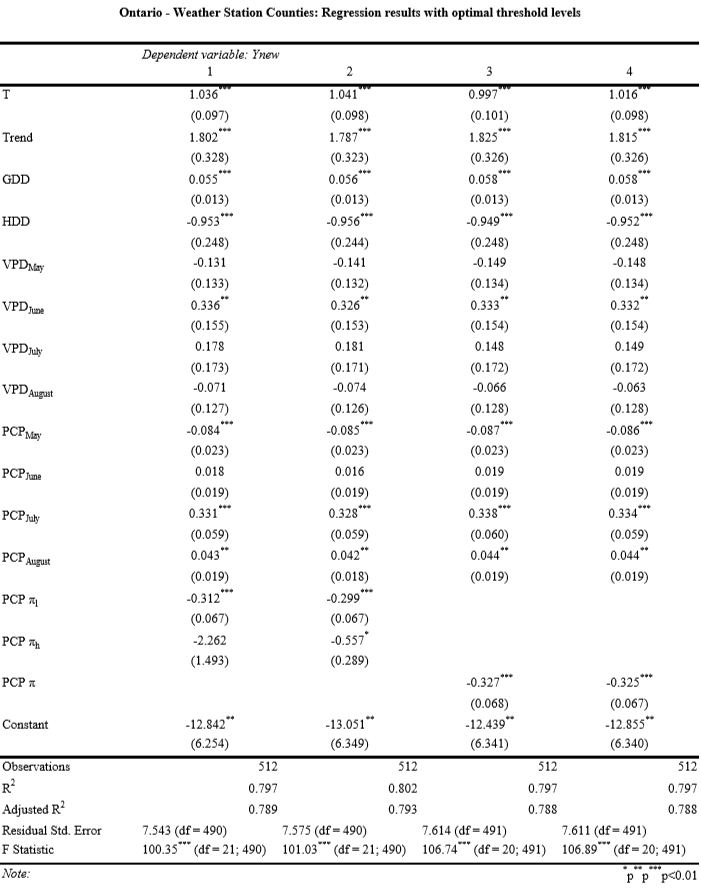
\includegraphics[width=1.0\textwidth]{Ontario_WSO_regression_results.png}
    \caption{Ontario - Weather Station Counties: Regression results with optimal threshold levels}
    \label{fig:my_label}
\end{table}

The model results from Iowa demonstrate the expected signs on all of the coefficients. The trend variable has a positive coefficient estimate as does GDD, while HDD, the variable representing potentially damaging high temperatures, has a negative coefficient with large magnitude. The Vapor Pressure Deficit (VPD) measure used is based on the difference between the saturated vapor pressure level at the maximum and minimum daily temperatures respectively. When the VPD levels are high, it indicates hot and dry conditions. Warm temperature with little moisture during planting and the early growth stages is generally beneficial for corn growth.  On the other hand, during the silking and pollination period crops are sensitive to extreme heat and water loss. During the end of the season the majority of growth is completed and the temperatures are becoming cooler. This leads to the expectation of a positive coefficient on beginning of season VPD, a negative coefficient on VPD during silking and pollination and a positive coefficient during the end of the season. All four of the results demonstrate these expected relationships in Iowa. The precipitation effect also changes throughout the growing season. In all four results, the sign on the $PCP_b$ variable, which corresponds to the beginning of the season when high levels of moisture can be damaging, is negative and small. During the silking stage the precipitation coefficients become positive and larger in magnitude which is consistent with the high levels of moisture required during this period. Finally, the end of season precipitation variable, $PCP_e$, is small and positive. Additionally, the silking stage precipitation threshold variable coefficients are both negative, as expected, given that the positive effect of precipitation in excess of the first threshold is expected to be small, and the effect of precipitation in excess of the second threshold is expected to be negative. Therefore, all of the coefficients are in the expected direction for all of the model estimates in Iowa. 

In the results for the province of Ontario and the three subsets considered, all of the coefficients had the expected signs except for the VPD coefficients. Otherwise, as in Iowa, the expected relationships are observed. In particular, the precipitation coefficients in July and the threshold coefficients have the expected signs and relative magnitudes. The general predicted yield climate relationship in Ontario and its subsets were very similar. Although the $R^2$ was higher among the smaller groups of counties which had more similarities, the general relationship was consistent across all of the models in terms of the sign and magnitudes of the parameter estimates. Given this observation, the remaining analysis is done only in reference to the group including all counties, and the subsets of the province are not considered further as they did not suggest a substantial difference in the effect of yield on climate by location.

\section{Precipitation Coefficient Estimates}

The precipitation coefficients are graphed versus precipitation level to demonstrate the implied effect of precipitation on yield. The coefficients are presented relative to the optimal threshold levels in 2000. The coefficient estimates obtained under each model and method are graphed together for each location.


\begin{figure}[H]
\centerfloat
 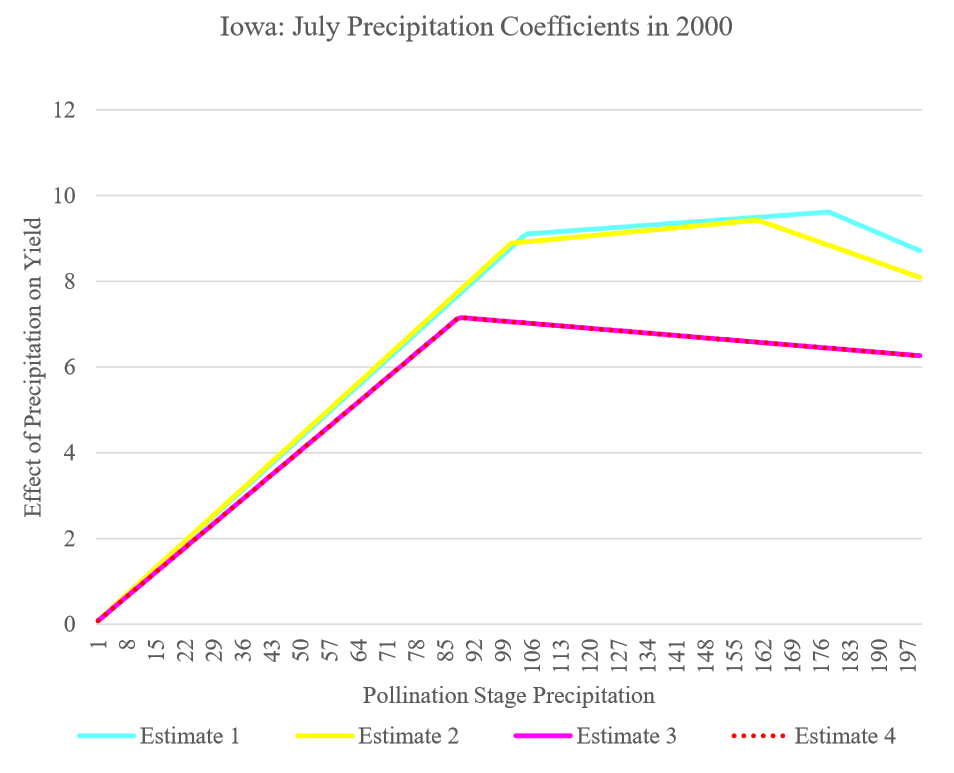
\includegraphics{Iowa_coefs.png}
    \caption{Iowa: Plot of Silking Stage Precipitation Coefficients using Threshold Levels from 2000}
\end{figure}

\begin{figure}[H]
 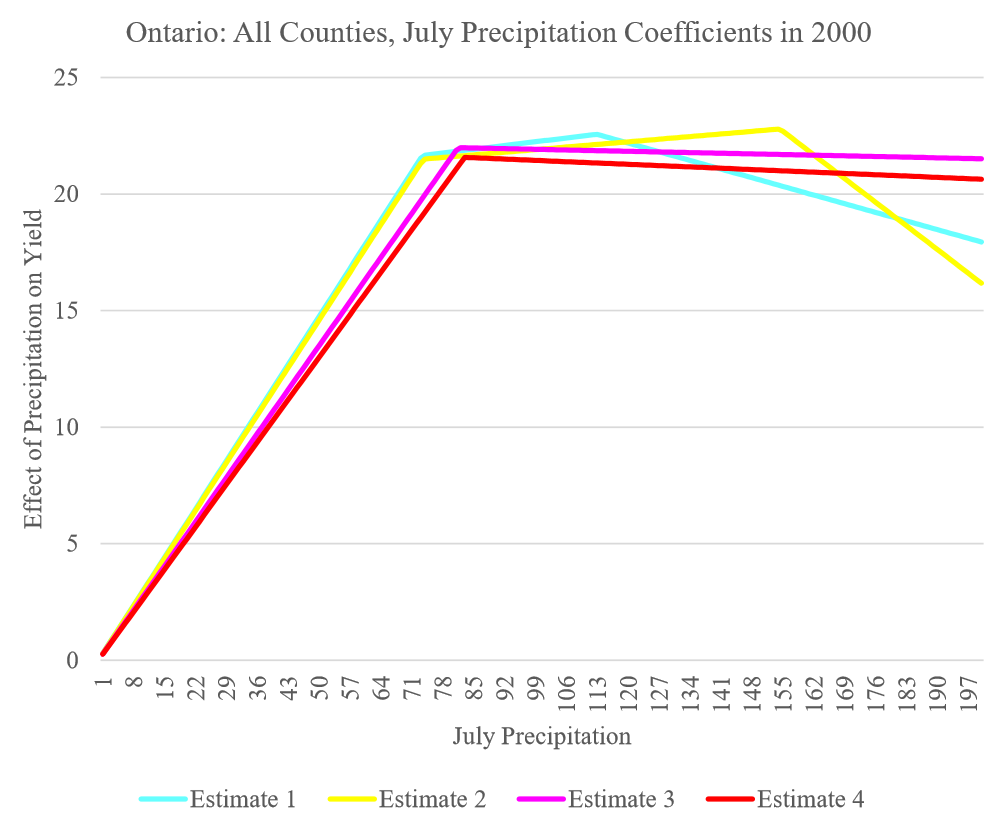
\includegraphics[width=\textwidth]{ON_coefs.png}
    \caption{Ontario: All Counties - Plot of July Precipitation Coefficients using Threshold Levels from 2000}
\end{figure}


\begin{figure}[H]
\centerfloat
 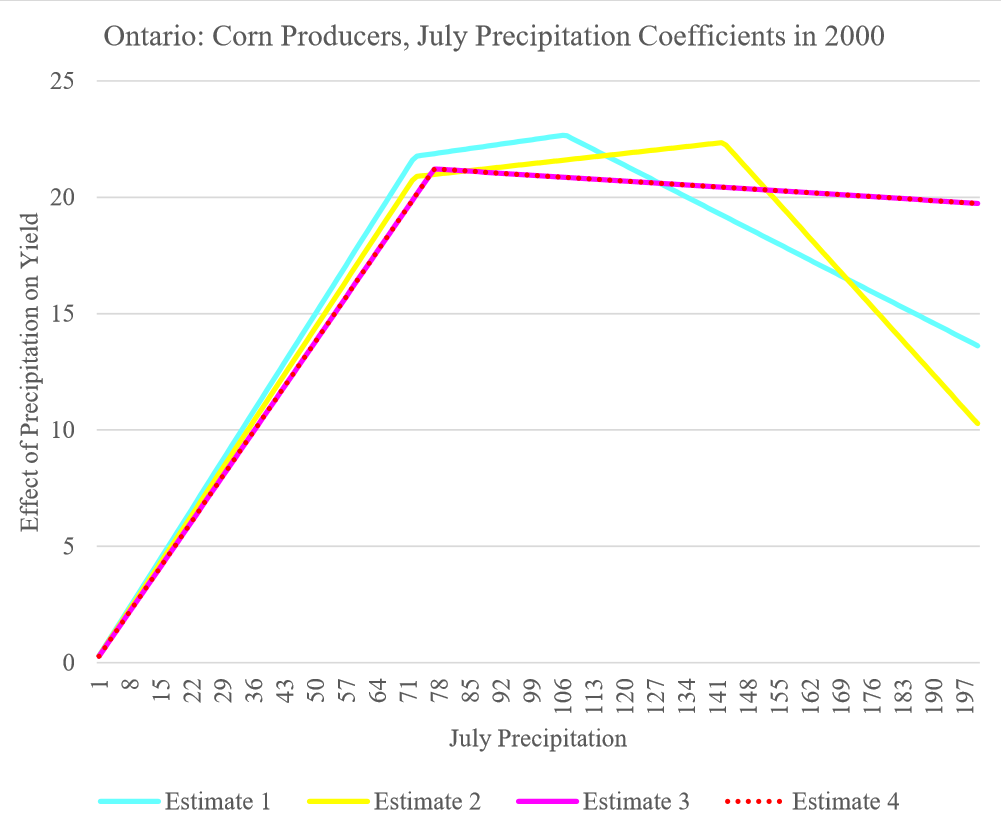
\includegraphics{trim_coefs.png}
    \caption{Ontario: Corn Producers - Plot of July Precipitation Coefficients using Threshold Levels from 2000}
\end{figure}

\begin{figure}[H]
\centerfloat
 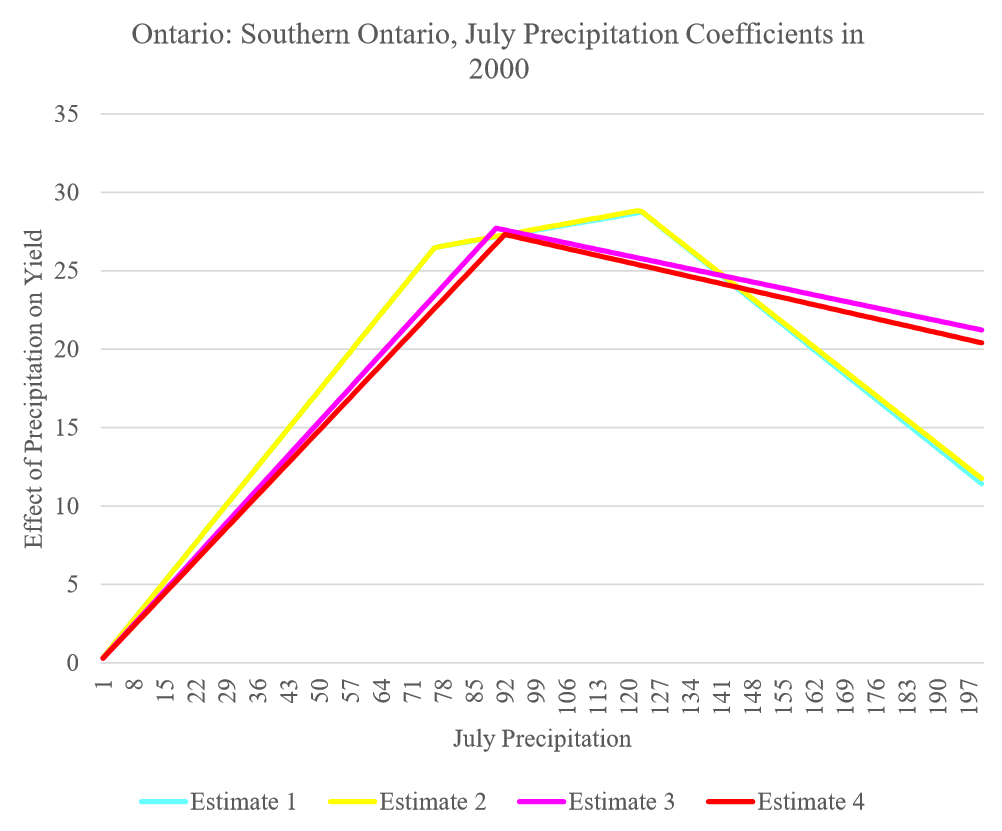
\includegraphics{SO_coefs.png}
    \caption{Southern Ontario - Plot of July Precipitation Coefficients using Threshold Levels from 2000}
\end{figure}

\begin{figure}[H]
\centerfloat
 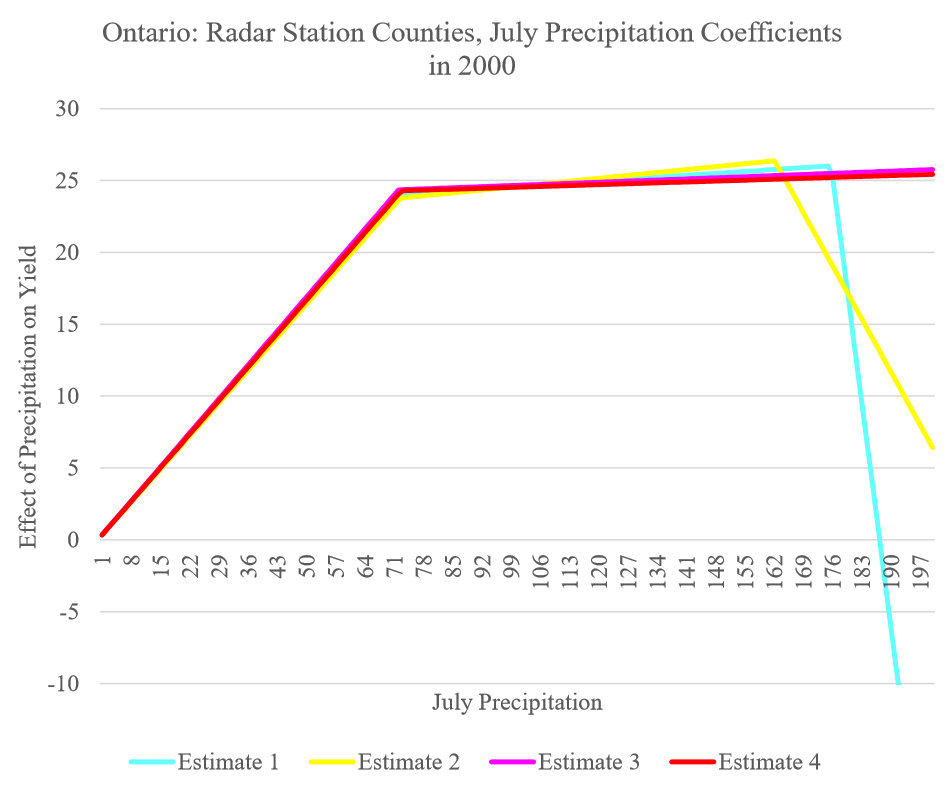
\includegraphics{WSO_coefs.png}
    \caption{Counties Near Ontario Radar Stations - Plot of July Precipitation Coefficients using Threshold Levels from 2000}
\end{figure}


The graphical presentation of the coefficients on silking stage precipitation levels demonstrates that they are consistent with the theoretical precipitation yield relationship. In all of the two threshold cases the implied effect of precipitation on yield, based on the estimated coefficients, is shown to be positive for small amounts of precipitation, then to start to level off after the first threshold, and finally to become negative after the second threshold. In the one threshold cases the implied effect begins positive and then decreases after the threshold level has been exceeded. These results fit well with the empirical framework that was developed, and fulfill the intuitive expectations regarding the effect of precipitation on yield during the silking and pollination stage.

\section{Threshold Results}

The optimal parameters controlling threshold levels estimated under each method and for each location are presented in the table below. 


\begin{table}[H]
\caption{Threshold Parameter Results by Location}
\label{my-label}
\begin{tabular}{lllllll}
\hline
 & $a_l$ & $b_l$ & $a_h$ & $b_h$ & $a$ & $b$ \\
\hline
 Iowa & & & & & & \\
\hline
1  & 60.416  & 0.982759   & 345.1  & -3.71379    &  & \\
2  &  64.416 & 0.813793  & 288.1         & -2.83103     & &   \\
3  &  &   &          &      & 86.416 &   0.434483 \\
4   &  &   &          &      & 86.416 &   0.434483 \\
\hline
Ontario: All counties & & & & & & \\
\hline
1  & 12 &  1.228125   & 137.25   &  -0.4875    &  & \\
2  &  13 & 1.2125  & 121.25         & 0.6625     & &   \\
3  &  &   &          &      & 3 &  1.56875 \\
4   &  &   &          &      & 10 &   1.4593753 \\
\hline
 Ontario: Corn Prducers & & & & & & \\
\hline
1  & 8 &  1.290625   & 140.99    &  -0.6875   &  & \\
2  &  8 & 1.290625  & 121.99      & 0.409375     & &   \\
3  &  &   &          &      & 5 &  1.4375 \\
4   &  &   &          &      & 5 &   1.4375 \\
\hline
 Southern Ontario & & & & & & \\
\hline
1  & 30.18 & 0.91875   & 118.37    &  0.09375   &  & \\
2  &  30.18 & 0.91875  & 116.37     & 0.125     & &   \\
3  &  &   &          &      & 32.18 &  1.15625 \\
4   &  &   &          &      & 34.18 &   1.15625 \\
\hline
Ontario: Radar Station Counties & & & & & & \\
\hline
1  &  10.06 & 1.253125   & 148.2    &  0.55    &  & \\
2  &   9.06 & 1.26875  & 132.2     & 0.6      & &   \\
3  &  &   &          &      & 7.06 &  1.3 \\
4   &  &   &          &      & 10.06 &    1.253125 \\
\hline
\end{tabular}
\end{table}



As shown in table 4.1, the results from the two threshold model in Iowa show that the lower threshold appears to be increasing through time while the upper threshold is decreasing. This result was found when the two threshold model was estimated both by method 1 and 2. The one threshold model results both showed the single knot to be increasing. 

The threshold results for all counties in Ontario generally show increasing thresholds over time. Estimate 1 shows a decreasing upper threshold over time, however, estimate 2 shows the upper threshold to be increasing. The one threshold model results both show the threshold to be increasing through time. The results for the ``Corn Producer" subset were very similar to those obtained for the entire province. The results for other two provincial subsets, ``Southern Ontario" and ``Weather Station Counties", showed all thresholds to be increasing under both models, and both estimation methods.

 The one threshold dynamic model results consistently showed that the precipitation threshold was increasing over time in all locations, and when estimated using both methods 1 and 2. The two threshold model estimation showed that the lower threshold appeared to be increasing over time and was generally similar to the level of the threshold estimates from the one threshold model.  The upper threshold, on the other hand, did not have consistent results; the direction of change over time depended on the location and method of estimation. Given that both the one and two threshold models had nearly equal fit, only the one threshold model is used for the remaining analysis due to its greater simplicity and consistency. The one threshold model was estimated using both methods 1 and 2. Method 2 requires the additional assumption that the correlation coefficient does not change when the threshold levels over time are modified. When estimating the model using method 2, the correlation coefficient does not have to be repeatedly calculated and therefore reduces computation time significantly. Only method 2 results will be used moving forward considering both the fact that a) the results obtained when estimating the model with methods 1 and 2 were almost identical and b) method 2 is less computationally expensive. 
 
 \section{Dynamic yield precipitation relationship}

The modelling of corn yield using historical county level data produced results that suggest that the yield-precipitation relationship is dynamic. In every location and location subset, the single threshold model estimation showed that the threshold value was increasing through time. 

To consider whether or not the relationship is in fact dynamic, a static yield precipitation model was also considered in Iowa and Ontario. This static model represents a restriction on the dynamic model as it forces the parameter controlling the threshold change over time to be equal to zero. The static and dynamic model results of interest are presented in tables below for both Iowa and Ontario. 


The dynamic and static models are compared in order to determine whether the dynamic model is significantly more likely to be correct as compared to the static model. The static model represents a restriction on the dynamic model which increases the degrees of freedom. The relative increase in the SSE under the static model versus the increased degrees of freedom is determined using an F-test. The static model has one additional degree of freedom since it essentially removes the threshold parameter $b$ which controls threshold change through time. The significance of $b$ is tested through this model comparison. The null hypothesis is that the two models are not statistically different, and therefore that $b$ is not significant. In Iowa, the F statistic computed was 6.051696, with 1 degree of freedom in the numerator and 5721 in the denominator, resulting in a p value of 0.0139 and implying that the threshold parameter $b$ is significant at the 95\% confidence level. In Ontario, the F statistic computed was  54.62528, with 1 degree of freedom in the numerator and 2001 in the denominator, resulting in a p value of less that 0.0001 and indicating that the threshold parameter $b$ is extremely significant in the yield model. These results support the hypothesis that the nature of the yield precipitation relationship is dynamic in both Iowa and Ontario.



% Table created by stargazer v.5.2 by Marek Hlavac, Harvard University. E-mail: hlavac at fas.harvard.edu
% Date and time: Mon, Dec 12, 2016 - 9:32:52 PM
% Requires LaTeX packages: dcolumn 
\begin{table}[!htbp] 
  \caption{Iowa: Optimal Threshold Dynamic and Static Yield Models} 
  \label{} 
\begin{tabular}{@{\extracolsep{5pt}}lD{.}{.}{-3} D{.}{.}{-3} } 
\\[-1.8ex]\hline 
\hline \\[-1.8ex] 
 & \multicolumn{2}{c}{\textit{Dependent variable: Ynew}} \\ 
\cline{2-3} 
\\[-1.8ex] 
 & \multicolumn{1}{c}{Dynamic} & \multicolumn{1}{c}{Static} \\ 
\\[-1.8ex] 
\hline \\[-1.8ex] 
 T & 1.852^{***} & 1.865^{***} \\ 
  & (0.090) & (0.090) \\ 
 GDD & 0.011^{***} & 0.010^{***} \\ 
  & (0.004) & (0.004) \\ 
 HDD & -0.040 & -0.039 \\ 
  & (0.030) & (0.030) \\ 
 VPD$_{b_i}$ & 0.110^{***} & 0.110^{***} \\ 
  & (0.021) & (0.021) \\  
 VPD$_{{pol}_i}$ & -0.333^{***} & -0.335^{***} \\ 
  & (0.044) & (0.045) \\  
 VPD$_{e_i}$ & 0.027^{*} & 0.028^{*} \\ 
  & (0.016) & (0.016) \\ 
 PCP$_{b_i}$ & -0.008^{***} & -0.008^{***} \\ 
  & (0.002) & (0.002) \\ 
 PCP$_{{pol}_i}$ & 0.081^{***} & 0.084^{***} \\ 
  & (0.007) & (0.007) \\ 
 PCP$_{e_i}$ & 0.005^{**} & 0.005^{**} \\ 
  & (0.003) & (0.003) \\ 
 PCP $\pi$ & -0.089^{***} & -0.089^{***} \\ 
  & (0.008) & (0.009) \\ 
 Constant & 2.430^{***} & 2.413^{***} \\ 
  & (0.361) & (0.362) \\ 
\hline \\[-1.8ex] 
Observations & \multicolumn{1}{c}{5,742} & \multicolumn{1}{c}{5,742} \\ 
R$^{2}$ & \multicolumn{1}{c}{0.140} & \multicolumn{1}{c}{0.140} \\ 
Adjusted R$^{2}$ & \multicolumn{1}{c}{0.137} & \multicolumn{1}{c}{0.137} \\ 
Residual Std. Error (df = 5723) & \multicolumn{1}{c}{6.581} & \multicolumn{1}{c}{6.584} \\ 
F Statistic (df = 18; 5723) & \multicolumn{1}{c}{50.318$^{***}$} & \multicolumn{1}{c}{50.206$^{***}$} \\ 
\hline 
\hline \\[-1.8ex] 
\textit{Note:}  & \multicolumn{2}{r}{$^{*}$p$<$0.1; $^{**}$p$<$0.05; $^{***}$p$<$0.01} \\ 
\end{tabular} 
\end{table} 



% Table created by stargazer v.5.2 by Marek Hlavac, Harvard University. E-mail: hlavac at fas.harvard.edu
% Date and time: Mon, Dec 12, 2016 - 7:11:51 AM
% Requires LaTeX packages: dcolumn 
\begin{table}[!htbp] 
  \caption{Ontario: Optimal Threshold Dynamic and Static Yield Models} 
  \label{} 
\begin{tabular}{@{\extracolsep{5pt}}lD{.}{.}{-3} D{.}{.}{-3} } 
\\[-1.8ex]\hline 
\hline \\[-1.8ex] 
 & \multicolumn{2}{c}{\textit{Dependent variable: Ynew}} \\ 
\cline{2-3} 
\\[-1.8ex] 
 & \multicolumn{1}{c}{Dynamic} & \multicolumn{1}{c}{Static} \\ 
\\[-1.8ex]
\hline \\[-1.8ex] 
 T & 0.796^{***} & 1.079^{***} \\ 
  & (0.056) & (0.043) \\ 
 Trend & 2.230^{***} & 2.055^{***} \\ 
  & (0.248) & (0.253) \\ 
 GDD & 0.037^{***} & 0.034^{***} \\ 
  & (0.007) & (0.008) \\ 
 HDD & -0.662^{***} & -0.657^{***} \\ 
  & (0.103) & (0.105) \\ 
 VPD$_{May}$ & -0.121 & -0.097 \\ 
  & (0.093) & (0.096) \\ 
 VPD$_{June}$ & 0.176^{*} & 0.152 \\ 
  & (0.094) & (0.096) \\ 
 VPD$_{July}$ & 0.077 & 0.118 \\ 
  & (0.100) & (0.104) \\ 
 VPD$_{Aug}$ & -0.205^{**} & -0.268^{***} \\ 
  & (0.092) & (0.094) \\ 
 PCP$_{May}$ & -0.024^{*} & -0.015 \\ 
  & (0.014) & (0.015) \\ 
 PCP$_{June}$ & 0.012 & 0.010 \\ 
  & (0.011) & (0.011) \\ 
 PCP$_{July}$ & 0.260^{***} & 0.110^{***} \\ 
  & (0.029) & (0.016) \\ 
 PCP$_{Aug}$ & 0.040^{***} & 0.036^{***} \\ 
  & (0.010) & (0.010) \\ 
 PCP $\pi$ & -0.268^{***} & -0.139^{***} \\ 
  & (0.032) & (0.028) \\ 
 Constant & 4.202^{*} & 4.110^{*} \\ 
  & (2.173) & (2.212) \\ 
\hline \\[-1.8ex] 
Observations & \multicolumn{1}{c}{2,048} & \multicolumn{1}{c}{2,048} \\ 
R$^{2}$ & \multicolumn{1}{c}{0.606} & \multicolumn{1}{c}{0.585} \\ 
Adjusted R$^{2}$ & \multicolumn{1}{c}{0.598} & \multicolumn{1}{c}{0.576} \\ 
Residual Std. Error (df = 2003) & \multicolumn{1}{c}{7.747} & \multicolumn{1}{c}{7.852} \\ 
F Statistic (df = 44; 2003) & \multicolumn{1}{c}{74.808$^{***}$} & \multicolumn{1}{c}{68.66$^{***}$} \\ 
\hline 
\hline \\[-1.8ex] 
\textit{Note:}  & \multicolumn{2}{r}{$^{*}$p$<$0.1; $^{**}$p$<$0.05; $^{***}$p$<$0.01} \\ 
\end{tabular} 
\end{table}



